We used micro-benchmarks to test the performance of RVM commits and RVM
recovery. To test commits, we allocated a number of pages, made modifications
to each one of them, and measured the time it took for \verb|rvm_txn_commit()|
to complete. To test recovery, we first allocate a number of pages and
close the connection to the server. We then restart the connection using the
recovery flag and time how long it takes \verb|rvm_cfg_create()| to complete.
When benchmarking the IB backend, we run three trials for each number of pages,
restarting the server after each trial.

\subsection{IB Backend}
Figure \ref{fig:ib-commit-ubm} shows the results of the commit micro-benchmark
using the IB backend. At the smallest page count, the commit time is around
150 microseconds. At 10K pages, the commit time has increased to 140 milliseconds.
As can be seen in the graph, the relation between page count and commit time
is fairly linear, with a slope of about 13.7 microseconds per page.

\begin{figure}[h]
    \caption{IB Commit Micro-Benchmark Results}
    \includegraphics[width=\linewidth]{graphs/commit-results-rm.pdf}
    \label{fig:ib-commit-ubm}
\end{figure}

Figure \ref{fig:ib-recovery-ubm} shows the results of the recovery
micro-benchmark using the IB backend. Recovery is quite a bit slower than
commit. Recovering a single page takes about 50 milliseconds, while recovering
10,000 pages takes more than 2 seconds. The relationship between number of
pages and recovery time is also not entirely linear.
The recovery time increases steadily until about 2000 pages, after which it
increases drastically. It is uncertain what is causing this sort of behavior,
as startup time involves a lot of different things, including the allocation
of local memory pages, receiving tag to address mappings from the server, and
copying data from the server.

\begin{figure}[h]
    \caption{IB Recovery Micro-Benchmark Results}
    \includegraphics[width=\linewidth]{graphs/recovery-results-rm.pdf}
    \label{fig:ib-recovery-ubm}
\end{figure}

\subsection{RAMCloud Backend}
\begin{figure}[t!]
\begin{center}
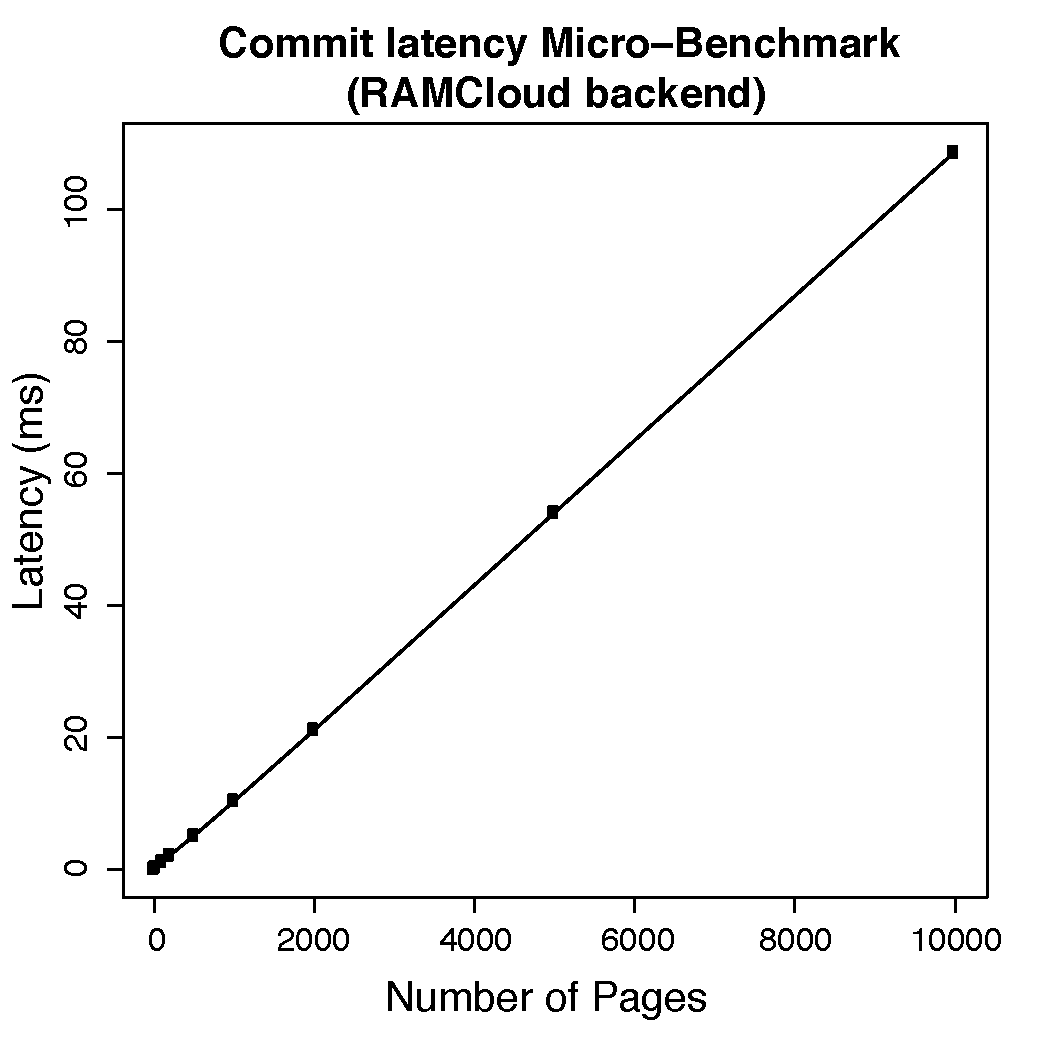
\includegraphics[scale=0.40]{graphs/commit_time_rc_latencies.pdf}
\end{center}
\caption{Commit time micro-benchmark when using the RAMCloud backend}
\label{fig:rc-commit-ubm}
\end{figure}

\subsection{RAMCloud Backend}
\begin{figure}[t!]
\begin{center}
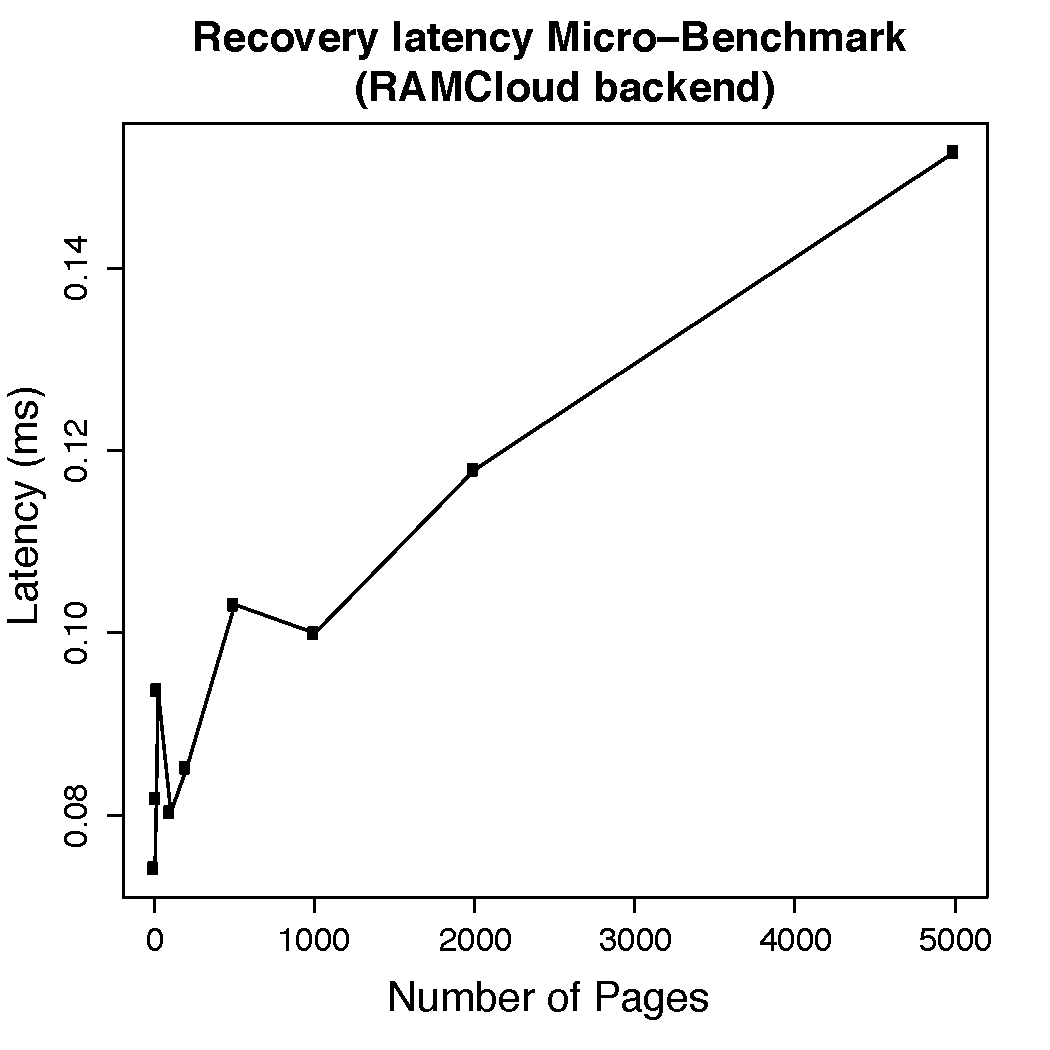
\includegraphics[scale=0.40]{graphs/recovery_time_rc_latencies.pdf}
\end{center}
\caption{Recovery time micro-benchmark when using the RAMCloud backend}
\label{fig:rc-recovery-ubm}
\end{figure}

Figure~\ref{fig:rc-commit-ubm} shows the results of the commit micro-benchmark when using the RAMCloud backend. 
The end-to-end latency of a commit operation is dominated by the number of pages to be commited, as each page write requires a round-trip to the RAMCloud server.
The RAMCloud backend also needs to save the table that contains the mapping between tags and keys in, but this only requires one interaction with the server.
The RAMCloud backend requires roughly 10 microseconds to write a page to RAMCloud. As can be seen in the graph, the commit time grows linearly with the number of pages as expected.





